\documentclass[12pt,a4paper]{article}

% ─── Page Layout ───────────────────────────────────────────────────────────────
\usepackage[a4paper, margin=0.8in, headheight=14pt]{geometry}

% ─── Fonts (XeLaTeX) ───────────────────────────────────────────────────────────
\usepackage{fontspec}
\usepackage{unicode-math}
\setmainfont{TeX Gyre Pagella}
\setmonofont[Scale=0.88]{TeX Gyre Cursor}
\setmathfont{Latin Modern Math}

% ─── Packages ──────────────────────────────────────────────────────────────────
\usepackage{xcolor}
\usepackage{colortbl}
\usepackage{titlesec}
\usepackage{enumitem}
\usepackage{tabularx}
\usepackage{booktabs}
\usepackage{array}
\usepackage{amsmath}
\usepackage{tikz}
\usetikzlibrary{shapes.geometric, arrows.meta, positioning, calc, fit, decorations.pathreplacing}
\usepackage{tcolorbox}
\tcbuselibrary{skins, breakable}
\usepackage{hyperref}
\usepackage{fancyhdr}
\usepackage{graphicx}
\usepackage{microtype}
\hyphenpenalty=10000
\exhyphenpenalty=10000
\sloppy
\usepackage{caption}
\usepackage{setspace}
\usepackage{multirow}
\usepackage{tocloft}

% ─── Q&A helper ────────────────────────────────────────────────────────────────
\newcommand{\Q}[1]{\textbf{#1}\par\noindent\ignorespaces}

% ─── Colour Palette ────────────────────────────────────────────────────────────
\definecolor{myred}{RGB}{196,30,58}
\definecolor{mydark}{RGB}{30,30,50}
\definecolor{mygreen}{RGB}{14,120,80}
\definecolor{myteal}{RGB}{0,130,140}
\definecolor{myamber}{RGB}{180,100,0}
\definecolor{mypurple}{RGB}{100,30,160}
\definecolor{mygray}{RGB}{246,247,249}
\definecolor{mgframe}{RGB}{180,185,200}
\definecolor{watermark}{RGB}{145,150,170}
\definecolor{hdrred}{RGB}{250,232,235}
\definecolor{hdrgreen}{RGB}{220,244,233}
\definecolor{hdrteal}{RGB}{220,242,244}
\definecolor{hdramber}{RGB}{253,242,215}
\definecolor{hdrpurple}{RGB}{238,228,255}
\definecolor{hdrgray}{RGB}{238,240,245}
\definecolor{rowalt}{RGB}{250,251,253}

% ─── Section Formatting ────────────────────────────────────────────────────────
\titleformat{\section}
  {\large\bfseries\color{myred}}{\thesection.}{0.5em}{}
  [\vspace{1pt}{\color{myred}\rule{\linewidth}{0.8pt}}]
\titleformat{\subsection}
  {\normalsize\bfseries\color{myteal}}{\thesubsection}{0.5em}{}
\titlespacing*{\section}{0pt}{18pt}{7pt}
\titlespacing*{\subsection}{0pt}{11pt}{4pt}

% ─── Paragraph ─────────────────────────────────────────────────────────────────
\setlength{\parindent}{0pt}
\setlength{\parskip}{4pt}

% ─── TOC Styling ───────────────────────────────────────────────────────────────
\renewcommand{\cfttoctitlefont}{\large\bfseries\color{myred}}
\renewcommand{\cftaftertoctitle}{\par\noindent{\color{myred}\rule{\linewidth}{0.8pt}}}
\setlength{\cftbeforetoctitleskip}{0pt}
\setlength{\cftaftertoctitleskip}{6pt}
\renewcommand{\cftsecfont}{\normalsize\bfseries\color{mydark}}
\renewcommand{\cftsecpagefont}{\normalsize\bfseries\color{mydark}}
\renewcommand{\cftsecleader}{\cftdotfill{\cftdotsep}}
\setlength{\cftbeforesecskip}{7pt}
\renewcommand{\cftsubsecfont}{\small\color{mydark}}
\renewcommand{\cftsubsecpagefont}{\small\color{mydark}}
\setlength{\cftbeforesubsecskip}{3pt}
\setlength{\cftsubsecindent}{1.4em}

% ─── Table helpers ─────────────────────────────────────────────────────────────
\renewcommand{\arraystretch}{1.45}
\setlength{\tabcolsep}{6pt}
\arrayrulecolor{mydark}
\newcolumntype{B}[1]{>{\small\bfseries\raggedright\arraybackslash}m{#1}}
\newcolumntype{Y}{>{\small\raggedright\arraybackslash}X}
\renewcommand{\tabularxcolumn}[1]{m{#1}}

% ─── Header / Footer ───────────────────────────────────────────────────────────
\pagestyle{fancy}
\fancyhf{}
\fancyhead[L]{\small\color{myred}\textbf{PE-EC702C}\;\color{mydark}--- Neural Network and Fuzzy Logic Control}
\fancyhead[R]{\small\color{myteal}\textbf{Module 3 Notes}}
\fancyfoot[C]{\small\color{mydark}\thepage}
\fancyfoot[R]{\small\color{watermark}\textit{\copyright\ Biraj}}
\renewcommand{\headrulewidth}{0.5pt}
\renewcommand{\footrulewidth}{0.3pt}

% ─── Hyperref ──────────────────────────────────────────────────────────────────
\hypersetup{
  colorlinks=true, linkcolor=myteal, urlcolor=myteal,
  pdfauthor={Biraj Sarkar},
  pdftitle={PE-EC702C --- Module 3 Notes}
}

% ─── tcolorbox styles ──────────────────────────────────────────────────────────
\tcbset{
  tikzbox/.style={
    colback=mygray, colframe=mgframe, boxrule=0.6pt, arc=4pt,
    left=8pt, right=8pt, top=6pt, bottom=6pt,
    colbacktitle=mgframe, coltitle=mydark,
    fonttitle=\small\bfseries
  },
  defbox/.style={
    colback=hdrgreen, colframe=mygreen, boxrule=0.8pt, arc=4pt,
    left=9pt, right=9pt, top=6pt, bottom=6pt,
    colbacktitle=mygreen, coltitle=white,
    fonttitle=\small\bfseries
  },
  formulabox/.style={
    colback=hdrteal, colframe=myteal, boxrule=0.8pt, arc=4pt,
    left=9pt, right=9pt, top=7pt, bottom=7pt,
    colbacktitle=myteal, coltitle=white,
    fonttitle=\small\bfseries
  },
  examplebox/.style={
    colback=hdramber, colframe=myamber, boxrule=0.8pt, arc=4pt,
    left=9pt, right=9pt, top=6pt, bottom=6pt,
    colbacktitle=myamber, coltitle=white,
    fonttitle=\small\bfseries,
    breakable
  },
  masonbox/.style={
    colback=hdrpurple, colframe=mypurple, boxrule=0.8pt, arc=4pt,
    left=9pt, right=9pt, top=6pt, bottom=6pt,
    colbacktitle=mypurple, coltitle=white,
    fonttitle=\small\bfseries
  },
  exambox/.style={
    colback=hdrpurple, colframe=mypurple, boxrule=1pt, arc=5pt,
    left=10pt, right=10pt, top=8pt, bottom=8pt,
    colbacktitle=mypurple, coltitle=white,
    fonttitle=\bfseries,
    breakable, title after break={\textbf{Frequently Asked / Viva Questions (contd.)}}}
}
\tcbset{breakable}

% ─── TikZ styles ───────────────────────────────────────────────────────────────
\tikzset{
  block/.style={rectangle, draw=myteal, fill=hdrteal,
    text width=2.2cm, align=center, minimum height=0.85cm,
    font=\small, rounded corners=3pt, line width=0.7pt},
  arrow/.style={-Stealth, thick, color=mydark},
  line/.style={thick, color=mydark}
}

% ═══════════════════════════════════════════════════════════════════════════════
\begin{document}
% ═══════════════════════════════════════════════════════════════════════════════

\begin{center}
  {\LARGE\bfseries\color{myred} PE-EC702C --- Neural Network \& Fuzzy Logic Control}\\[5pt]
  {\normalsize\color{mydark} Semester VII \quad$\bullet$\quad 3L:0T:0P \quad$\bullet$\quad 3 Credits}\\[3pt]
  {\normalsize\color{myteal}\textbf{Module 3 Exam Notes: Adaptive Resonance \& Backpropagation}}\\[3pt]
  {\small\color{mydark} CGEC \;$|$\; B.Tech ECE (2023--27) \;$|$\; \textit{Biraj Sarkar}}
\end{center}
\vspace{2pt}
\noindent{\color{myred}\rule{\linewidth}{1.5pt}}
\vspace{2pt}

\hypersetup{linkcolor=mydark}
\tableofcontents
\hypersetup{linkcolor=myteal}
\newpage

% ===============================================================================
\section{Backpropagation Neural Networks (BPNN)}
% ===============================================================================

The Backpropagation algorithm is the standard method for training Multi-Layer Perceptrons (MLPs). It is a supervised learning method based on the generalized delta rule (gradient descent on error space).

\begin{tcolorbox}[defbox, title={Multi-Layer Perceptron (MLP)}]
A \textbf{Multi-Layer Perceptron (MLP)} is a feedforward artificial neural network topology consisting of an input layer, one or more hidden layers, and an output layer of non-linear processing units.
\end{tcolorbox}

\begin{tcolorbox}[tikzbox, title={Multi-Layer Perceptron Feedforward Architecture}]
\centering
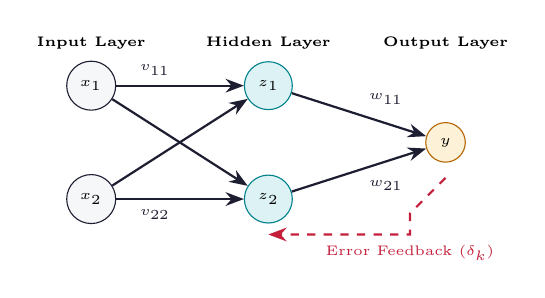
\begin{tikzpicture}[scale=0.9, every node/.style={font=\tiny}]
  % Input Layer
  \node[circle, draw=mydark, fill=mygray, minimum size=0.5cm] (x1) at (-2.5, 0.8) {$x_1$};
  \node[circle, draw=mydark, fill=mygray, minimum size=0.5cm] (x2) at (-2.5, -0.8) {$x_2$};
  \node at (-2.5, 1.4) {\textbf{Input Layer}};

  % Hidden Layer
  \node[circle, draw=myteal, fill=hdrteal, minimum size=0.5cm] (z1) at (0, 0.8) {$z_1$};
  \node[circle, draw=myteal, fill=hdrteal, minimum size=0.5cm] (z2) at (0, -0.8) {$z_2$};
  \node at (0, 1.4) {\textbf{Hidden Layer}};

  % Output Layer
  \node[circle, draw=myamber, fill=hdramber, minimum size=0.5cm] (y) at (2.5, 0) {$y$};
  \node at (2.5, 1.4) {\textbf{Output Layer}};

  % Connections: Input to Hidden
  \draw[arrow] (x1) -- node[midway, above left] {$v_{11}$} (z1);
  \draw[arrow] (x1) -- (z2);
  \draw[arrow] (x2) -- (z1);
  \draw[arrow] (x2) -- node[midway, below left] {$v_{22}$} (z2);

  % Connections: Hidden to Output
  \draw[arrow] (z1) -- node[midway, above right] {$w_{11}$} (y);
  \draw[arrow] (z2) -- node[midway, below right] {$w_{21}$} (y);
  
  % Error propagation path
  \draw[dashed, arrow, color=myred] (2.5, -0.5) -- +(-0.5, -0.5) |- (0, -1.3) node[midway, below] {Error Feedback ($\delta_k$)};
\end{tikzpicture}
\end{tcolorbox}

\subsection{Derivation of the Backpropagation Learning Rules}
Let $E$ be the total sum-of-squares error over the output units:
\begin{equation}
  E = \frac{1}{2} \sum_{k} (t_k - y_k)^2
\end{equation}
where $t_k$ is the target output and $y_k$ is the computed activation of output unit $k$.
The activation function used is the binary sigmoid:
\begin{equation}
  y_k = f(net_k) = \frac{1}{1 + e^{-net_k}} \quad \rightarrow \quad f'(net_k) = y_k(1 - y_k)
\end{equation}
where $net_k = \sum_{j} w_{kj} z_j + b_k$ ($z_j$ is the activation of hidden node $j$).

\par\noindent
Using gradient descent, the weight changes are proportional to the negative gradient of error:
\begin{equation}
  \Delta w_{kj} = -\eta \frac{\partial E}{\partial w_{kj}}
\end{equation}
By applying the chain rule of calculus:
\begin{equation}
  \frac{\partial E}{\partial w_{kj}} = \frac{\partial E}{\partial y_k} \cdot \frac{\partial y_k}{\partial net_k} \cdot \frac{\partial net_k}{\partial w_{kj}}
\end{equation}
Evaluating each derivative:
\begin{equation*}
  \frac{\partial E}{\partial y_k} = -(t_k - y_k), \quad \frac{\partial y_k}{\partial net_k} = f'(net_k) = y_k(1 - y_k), \quad \frac{\partial net_k}{\partial w_{kj}} = z_j
\end{equation*}
Substituting these terms back:
\begin{equation}
  \frac{\partial E}{\partial w_{kj}} = -(t_k - y_k) f'(net_k) z_j
\end{equation}
Defining the error term (delta) for output unit $k$ as $\delta_k = (t_k - y_k) f'(net_k)$:
\begin{equation}
  \Delta w_{kj} = \eta \delta_k z_j
\end{equation}

\par\noindent
For input-to-hidden weights $v_{ji}$ connecting input $i$ to hidden unit $j$:
\begin{equation}
  \Delta v_{ji} = -\eta \frac{\partial E}{\partial v_{ji}} = -\eta \frac{\partial E}{\partial z_j} \cdot \frac{\partial z_j}{\partial net_j} \cdot \frac{\partial net_j}{\partial v_{ji}}
\end{equation}
where $z_j = f(net_j)$ and $net_j = \sum_i v_{ji} x_i + b_j$.
The error gradient relative to hidden activation $z_j$ accumulates from all output nodes:
\begin{equation*}
  \frac{\partial E}{\partial z_j} = \sum_k \frac{\partial E}{\partial net_k} \cdot \frac{\partial net_k}{\partial z_j} = \sum_k (-\delta_k) w_{kj}
\end{equation*}
Applying the other terms:
\begin{equation*}
  \frac{\partial z_j}{\partial net_j} = f'(net_j) = z_j(1 - z_j), \quad \frac{\partial net_j}{\partial v_{ji}} = x_i
\end{equation*}
Defining the error term (delta) for hidden unit $j$ as $\delta_j = f'(net_j) \sum_k \delta_k w_{kj}$:
\begin{equation}
  \Delta v_{ji} = \eta \delta_j x_i
\end{equation}

% ===============================================================================
\section{Adaptive Resonance Theory (ART)}
% ===============================================================================

Developed by Stephen Grossberg and Gail Carpenter (1987), ART is designed to solve the stability-plasticity dilemma in unsupervised neural networks.

\begin{tcolorbox}[defbox, title={Stability-Plasticity Dilemma}]
\textbf{Stability-Plasticity Dilemma:} The challenge of designing a learning system that remains adaptive to new patterns (plasticity) while preventing new learning from washing out previously acquired knowledge (stability).
\end{tcolorbox}

\subsection{ART1 vs. ART2}
\begin{itemize}[leftmargin=*, itemsep=3pt]
  \item \textbf{ART1:} Designed to process binary input vectors ($\{0, 1\}$).
  \item \textbf{ART2:} Designed to process continuous (analog) input vectors.
\end{itemize}

\subsection{ART1 Architecture and Operation}
ART1 consists of two subsystems: the Attentional Subsystem and the Orienting Subsystem.

\begin{tcolorbox}[tikzbox, title={ART1 Network Architecture}]
\centering
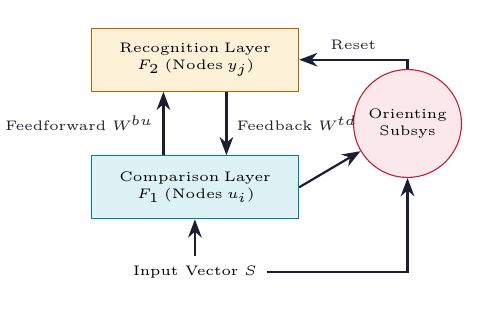
\begin{tikzpicture}[scale=0.9, every node/.style={font=\tiny}]
  % Comparison Layer (F1)
  \node[rectangle, draw=myteal, fill=hdrteal, text width=2.4cm, align=center, minimum height=0.8cm] (f1) at (0, 0) {Comparison Layer\\$F_1$ (Nodes $u_i$)};
  
  % Recognition Layer (F2)
  \node[rectangle, draw=myamber, fill=hdramber, text width=2.4cm, align=center, minimum height=0.8cm] (f2) at (0, 1.8) {Recognition Layer\\$F_2$ (Nodes $y_j$)};

  % Orienting Subsystem (Reset)
  \node[circle, draw=myred, fill=hdrred, minimum size=0.8cm, align=center] (orient) at (3.0, 0.9) {Orienting\\Subsys};

  % Feedback and Feedforward arrows
  \draw[arrow, transform canvas={xshift=-0.4cm}] (f1.north) -- node[midway, left] {Feedforward $W^{bu}$} (f2.south);
  \draw[arrow, transform canvas={xshift=0.4cm}] (f2.south) -- node[midway, right] {Feedback $W^{td}$} (f1.north);

  % Inputs
  \node (in) at (0, -1.2) {Input Vector $S$};
  \draw[arrow] (in) -- (f1);

  % Vigilance comparison
  \draw[arrow] (in.east) -| (orient);
  \draw[arrow] (f1.east) -- (orient);
  \draw[arrow] (orient.north) |- (f2.east) node[near end, above] {Reset};
\end{tikzpicture}
\end{tcolorbox}

\par\noindent
\textbf{Working Mechanism:}
\begin{enumerate}[leftmargin=*, itemsep=2.5pt]
  \item \textbf{Input presentation:} Input $S$ is sent to the $F_1$ layer.
  \item \textbf{Feedforward activation:} $F_1$ transmits the pattern to the $F_2$ layer. The $F_2$ layer is a competitive layer where the node with the highest net input wins (winner-take-all).
  \item \textbf{Feedback Template matching:} The winning $F_2$ neuron projects its prototype vector (template) back down to $F_1$.
  \item \textbf{Vigilance Test:} The orienting subsystem calculates the ratio of match:
    \begin{equation}
      \frac{|S \cap X|}{|S|}
    \end{equation}
    where $X$ is the activation of the $F_1$ layer.
    \begin{itemize}[leftmargin=1.5em, itemsep=1.5pt]
      \item If ratio $\ge \rho$ (vigilance parameter), \textbf{resonance} occurs. The network accepts the match and updates the winning neuron's weights.
      \item If ratio $< \rho$, the orienting subsystem sends a \textbf{reset signal} to temporarily disable the winning $F_2$ node. The search process repeats for other $F_2$ nodes. If no match is found, a new category node is initialized.
    \end{itemize}
\end{enumerate}

% ===============================================================================
\section{Boltzmann Machine Learning}
% ===============================================================================

The Boltzmann Machine is a recurrent, symmetrically connected network consisting of stochastic binary units (visible and hidden) that operate under statistical thermodynamics principles.

\begin{tcolorbox}[formulabox, title={Boltzmann Energy \& Transition Rules}]
The total energy $E$ of a Boltzmann state configuration is defined as:
\begin{equation}
  E = -\sum_{i < j} w_{ij} s_i s_j - \sum_{i} \theta_i s_i
\end{equation}
where $w_{ij}$ is the connection weight, $s_i \in \{0, 1\}$ is the state of unit $i$, and $\theta_i$ is the threshold bias.
\par\noindent
The probability that unit $i$ transitions to state $s_i = 1$ is given by the sigmoid-like logistic function:
\begin{equation}
  P(s_i = 1) = \frac{1}{1 + e^{-\Delta E_i / T}}
\end{equation}
where $\Delta E_i = \sum_j w_{ij} s_j + \theta_i$ is the energy difference and $T$ is the temperature parameter.
\end{tcolorbox}

\subsection{Boltzmann Learning Rule}
Boltzmann training occurs in two distinct phases:
\begin{enumerate}[leftmargin=*, itemsep=3.5pt]
  \item \textbf{Positive (Clamped) Phase:} The visible units are clamped to target training patterns. The network is allowed to reach thermal equilibrium, and the correlation probabilities $p_{ij}^+$ that units $i$ and $j$ are active simultaneously are measured.
  \item \textbf{Negative (Free-Running) Phase:} No units are clamped. The network runs freely to reach thermal equilibrium, and the free probabilities $p_{ij}^-$ are measured.
  \item \textbf{Weight Update:} Weights are updated to minimize Kullback-Leibler divergence:
    \begin{equation}
      \Delta w_{ij} = \eta (p_{ij}^+ - p_{ij}^-)
    \end{equation}
\end{enumerate}

% ===============================================================================
\section{Worked Examples}
% ===============================================================================

\begin{tcolorbox}[examplebox, title={Backpropagation Step-by-Step Numerical}]
\textbf{Problem:} Consider a simplified neural network containing 1 input node ($x$), 1 hidden node ($z$), and 1 output node ($y$). The transfer function is the binary sigmoid: $f(net) = 1/(1 + e^{-net})$. 
\par
Given: Input $x = 1.0$, target $t = 0.9$, learning rate $\eta = 0.5$.
Initial weights and biases:
\begin{itemize}[leftmargin=*, itemsep=2pt]
  \item Input-to-hidden weight $v = 0.5$, bias $b_1 = 0.2$
  \item Hidden-to-output weight $w = 0.8$, bias $b_2 = 0.1$
\end{itemize}
Calculate the updated weights $w$ and $v$ after a single backpropagation epoch.
\par\vspace{4pt}\noindent\rule{\linewidth}{0.5pt}\par
\textbf{Solution:}

\textbf{1. Forward Pass:}
\begin{itemize}[leftmargin=*, itemsep=2.5pt]
  \item \textbf{Hidden Node $z$:}
    \begin{align*}
      net_z &= v \cdot x + b_1 = 0.5(1.0) + 0.2 = 0.7 \\
      z &= f(net_z) = \frac{1}{1 + e^{-0.7}} \approx 0.668
    \end{align*}
  \item \textbf{Output Node $y$:}
    \begin{align*}
      net_y &= w \cdot z + b_2 = 0.8(0.668) + 0.1 \approx 0.634 \\
      y &= f(net_y) = \frac{1}{1 + e^{-0.634}} \approx 0.653
    \end{align*}
\end{itemize}

\par\vspace{4pt}
\textbf{2. Backward Pass (Error Propagation):}
\begin{itemize}[leftmargin=*, itemsep=2.5pt]
  \item \textbf{Output Delta ($\delta_y$):}
    \begin{align*}
      \delta_y &= (t - y) y (1 - y) \\
      &= (0.9 - 0.653) \cdot 0.653 \cdot (1 - 0.653) \\
      &= 0.247 \cdot 0.653 \cdot 0.347 \approx 0.0560
    \end{align*}
  \item \textbf{Hidden Delta ($\delta_z$):}
    \begin{align*}
      \delta_z &= \delta_y \cdot w \cdot z(1 - z) \\
      &= 0.0560 \cdot 0.8 \cdot 0.668 \cdot (1 - 0.668) \\
      &= 0.0448 \cdot 0.668 \cdot 0.332 \approx 0.00993
    \end{align*}
\end{itemize}

\par\vspace{4pt}
\textbf{3. Weight Updates:}
\begin{itemize}[leftmargin=*, itemsep=2.5pt]
  \item \textbf{Hidden-to-Output Weight ($w$):}
    \begin{align*}
      \Delta w &= \eta \cdot \delta_y \cdot z = 0.5 \cdot 0.0560 \cdot 0.668 \approx 0.0187 \\
      w(new) &= 0.8 + 0.0187 = 0.8187
    \end{align*}
  \item \textbf{Input-to-Hidden Weight ($v$):}
    \begin{align*}
      \Delta v &= \eta \cdot \delta_z \cdot x = 0.5 \cdot 0.00993 \cdot 1.0 \approx 0.00497 \\
      v(new) &= 0.5 + 0.00497 = 0.50497
    \end{align*}
\end{itemize}
The updated weights are $w \approx 0.8187$ and $v \approx 0.5050$.
\end{tcolorbox}

\newpage

% ===============================================================================
% MANDATORY QUICK REVISION PAGE
% ===============================================================================
\begin{center}
  {\large\bfseries\color{myred} Quick Revision --- Module III}\\[3pt]
  {\small\color{mydark} Adaptive Resonance \& Backpropagation $|$ PE-EC702C}
\end{center}
\noindent{\color{myred}\rule{\linewidth}{1.2pt}}
\vspace{4pt}

\begin{tcolorbox}[formulabox, title={\textbf{Key Formulas at a Glance}}]
\renewcommand{\arraystretch}{1.3}
\begin{tabularx}{\linewidth}{B{5.0cm} X}Total Output Error & $E = \frac{1}{2} \sum_{k} (t_k - y_k)^2$ \\
Output Layer Delta ($\delta_k$) & $\delta_k = (t_k - y_k) y_k (1 - y_k) \quad \text{(for sigmoid)}$ \\
Hidden Layer Delta ($\delta_j$) & $\delta_j = z_j(1 - z_j) \sum_{k} \delta_k w_{kj} \quad \text{(for sigmoid)}$ \\
BPNN Weight Updates & $\Delta w_{kj} = \eta \delta_k z_j, \quad \Delta v_{ji} = \eta \delta_j x_i$ \\
ART1 Vigilance Ratio & Match $= \frac{|S \cap X|}{|S|} \ge \rho \quad \text{(where } \rho \in [0, 1]\text{)}$ \\
Boltzmann Energy Configuration & $E = -\sum_{i < j} w_{ij} s_i s_j - \sum_i \theta_i s_i$
\end{tabularx}
\end{tcolorbox}

\begin{tcolorbox}[defbox, title={\textbf{One-Line Definitions}}]
\begin{itemize}[leftmargin=*, itemsep=2.5pt, topsep=0pt]
  \item \textbf{Backpropagation:} A supervised gradient-descent algorithm that updates network weights to minimize the sum of squared errors.
  \item \textbf{Stability-Plasticity Dilemma:} The goal of learning new input patterns without overwriting previously learned representations.
  \item \textbf{Vigilance Parameter ($\rho$):} The threshold parameter in ART that determines how closely an input must match a category template.
  \item \textbf{Resonance:} The state in ART where an input matches a template well enough to initiate weight tuning.
  \item \textbf{Boltzmann Machine:} A recurrent stochastic neural network that uses simulated annealing to escape local energy minima.
\end{itemize}
\end{tcolorbox}

\begin{tcolorbox}[exambox, title={\textbf{Frequently Asked / Viva Questions}}]
\begin{enumerate}[leftmargin=*, itemsep=3.5pt, label=\arabic*.]
  \item \Q{Why is Backpropagation referred to as a "supervised" learning algorithm?} Because weight adjustments are calculated using the difference (error) between the network's computed output and the target (label) vector.
  \item \Q{State the purpose of the activation function's derivative $f'(net)$ in backpropagation.} It scales the weight update based on the slope of the activation curve. In flat regions (near $0$ or $1$ for sigmoids), updates are very small, preventing oscillations.
  \item \Q{What is the effect of setting a high vigilance parameter ($\rho$) in ART1?} A high vigilance value (e.g. $\rho = 0.95$) requires highly precise matches, leading the network to create many narrow, fine-grained categories.
  \item \Q{What is the effect of setting a low vigilance parameter ($\rho$) in ART1?} A low vigilance value (e.g. $\rho = 0.3$) allows loose matching, causing the network to group highly different inputs into a few broad, coarse categories.
  \item \Q{How does Boltzmann learning utilize the positive and negative phases?} The positive phase clamps inputs to capture target correlations ($p_{ij}^+$), while the negative phase runs freely to capture network-generated correlations ($p_{ij}^-$).
  \item \Q{Why does backpropagation sometimes get stuck in local minima?} Because gradient descent follows local gradients on the error surface. If it enters a local valley (minimum) that is not the absolute lowest point (global minimum), it cannot escape.
  \item \Q{What is the function of the orienting subsystem in ART1?} It acts as a controller that compares the input match ratio with the vigilance parameter $\rho$. If it is too low, it issues a reset signal to disable the winning category node.
  \item \Q{Define the term "Simulated Annealing" in Boltzmann machines.} The process of starting at a high temperature $T$ to allow stochastic state jumps (escaping local minima), and slowly cooling down to settle in the global minimum state.
  \item \Q{What is the difference between feedforward and feedback networks in terms of stability?} Feedforward networks compute outputs instantaneously and are always stable. Feedback networks have recurrent loop dynamics and can oscillate or require iterative convergence to reach stability.
  \item \Q{Why is $\frac{1}{2}$ added in the error formulation $E = \frac{1}{2}\sum(t-y)^2$?} It is a mathematical convenience that cancels out the coefficient $2$ when taking the derivative $\frac{\partial E}{\partial y} = -(t-y)$ during gradient calculations.
\end{enumerate}
\tcbset{colbacktitle=myteal, coltitle=white}
\end{tcolorbox}

\begin{tcolorbox}[tikzbox, title={Comparison of Adaptive Architectures}]
\centering
{\renewcommand{\arraystretch}{1.55}%
\begin{tabularx}{\linewidth}{|>{\bfseries}B{3.2cm}|Y|Y|Y|}
\hline
Attribute & Backpropagation BPNN & ART1 & Boltzmann Machine \\
\hline
Learning Type & Supervised & Unsupervised & Supervised / Unsupervised \\
\hline
Connections & Feedforward only & Bidirectional (top-down/bottom-up) & Symmetric recurrent loops \\
\hline
Neuron States & Analog / Continuous & Binary $\{0, 1\}$ & Stochastic Binary $\{0, 1\}$ \\
\hline
Page Resolution & Fixed classes & Dynamic category creation & Probability distribution fitting \\
\hline
\end{tabularx}}
\tcbset{colbacktitle=myteal, coltitle=white}
\end{tcolorbox}

\end{document}
